\usubsection{Tercer incremento}

El tercer incremento fue planificado con un doble propósito. Por una parte, se buscó incorporar un módulo de apoyo pedagógico que facilitara la introducción progresiva del usuario al lenguaje y al paradigma de flujos de datos. Por otra, se planteó el refinamiento de la interfaz del editor y la ampliación del modelo de distribución mediante abstracciones visuales de mayor nivel. Para ello, se definieron como objetivos el desarrollo del módulo de desafíos de aprendizaje, la reorganización visual del editor y la incorporación de nodos inspirados en operaciones colectivas de MPI.

\usubsubsection{Refinamiento de la interfaz de usuario del editor}

La implementación comenzó con el refinamiento de la interfaz del editor. Se incorporó una cabecera persistente con identidad visual, se reorganizaron los controles globales del sistema, se rediseñaron los botones de ejecución con colores semánticos, se optimizó la paleta de nodos para ceder mayor espacio al lienzo y se redefinió la geometría de los nodos para hacerla más compacta. También se mejoró la delimitación visual de la consola para distinguir con claridad el área de construcción lógica del área de salida.

El resultado de este refinamiento puede apreciarse en la figura \ref{fig:editor-incr2}, la cual ilustra el editor renovado, ofreciendo un entorno de trabajo más espacioso y estéticamente adaptado a las capacidades cognitivas y motoras del público objetivo.

\begin{figure}[H]
    \centering
    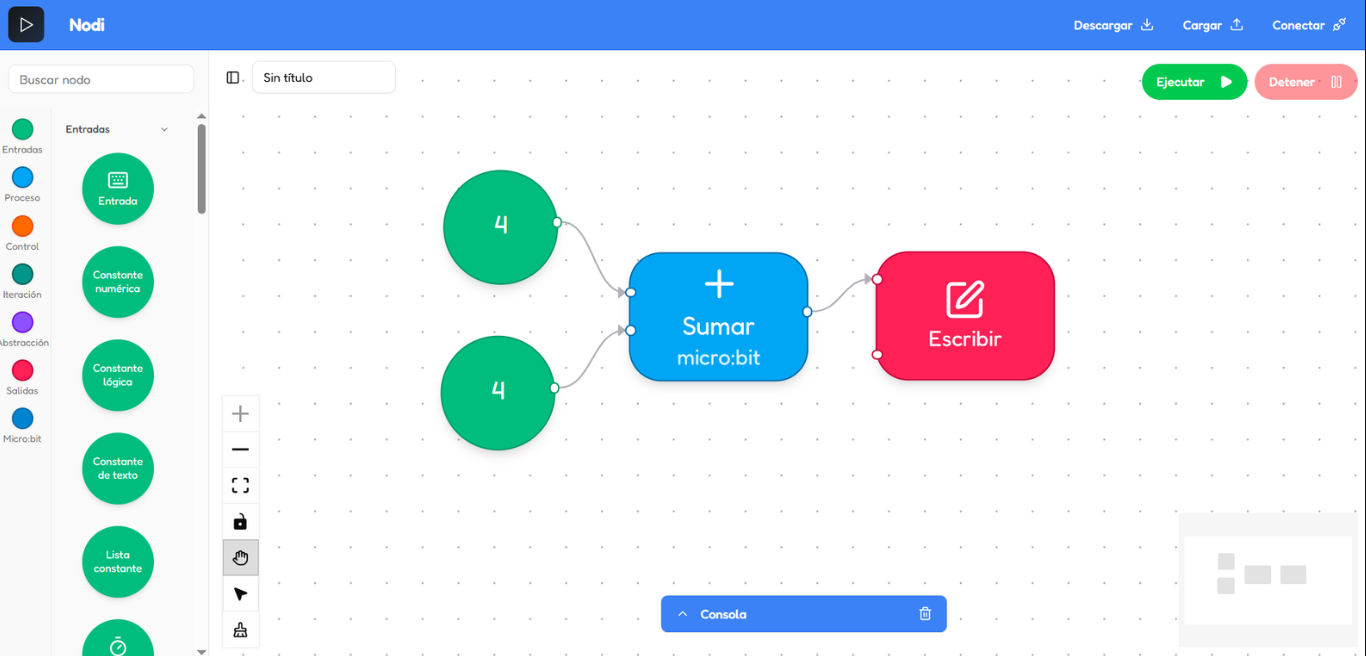
\includegraphics[width=\textwidth]{../images/editor-incr2.png}
    \caption[Interfaz del editor en el tercer incremento]{\normalfont Interfaz del editor renovado tras el refinamiento de la interfaz de usuario}
    \label{fig:editor-incr2}
\end{figure}

\usubsubsection{Módulo de desafíos}

El diseño de este módulo se fundamentó en principios de gamificación y psicología cognitiva. De acuerdo con \citeA{sandhu2013}, la gamificación consiste en utilizar el pensamiento y las dinámicas de los juegos para involucrar a las audiencias en la resolución de problemas. En el contexto del diseño de interfaces para niños, la inclusión de elementos gamificados basados en el aprendizaje resulta fundamental para fomentar la comprensión de conceptos abstractos. Bajo esta premisa, el módulo de desafíos se estructuró para proporcionar una ruta de aprendizaje interactiva e incremental.

Para asegurar la efectividad de los retos, los usuarios se clasificaron según los grupos definidos por Piaget en su teoría del desarrollo cognitivo. El grupo de 8 a 11 años, ubicado en la etapa de Operaciones Concretas, comprende la causalidad pero presenta dificultades ante conceptos puramente abstractos. Por tanto, sus desafíos emplean metáforas visuales manipulables donde la relación entrada-salida es fácilmente observable. En contraste, los jóvenes de 12 a 16 años, en la etapa de Operaciones Formales, poseen habilidades de razonamiento abstracto e hipotético-deductivo. En consecuencia, sus retos prescinden de las metáforas directas para introducir lógica compleja, requiriendo planificación algorítmica y manejo concurrente de variables.

Adicionalmente, para evitar la sobrecarga cognitiva en ambos grupos, el módulo implementa el principio de andamiaje. A diferencia del modo de creación libre, el entorno restringe dinámicamente la paleta de herramientas, exponiendo únicamente los nodos necesarios para resolver el nivel en curso. Esta decisión de diseño interactivo se alinea con los hallazgos de \citeA{bers2023} en Scratch-Jr, donde limitar deliberadamente los comandos disponibles resultó clave para no abrumar la carga cognitiva de los usuarios principiantes y focalizar su atención en la lógica.

Para complementar esto, se desarrolló un motor de validación que evalúa en tiempo real el flujo construido, comparando la salida final generada con el resultado esperado del reto para distintos casos de prueba. Esta validación emite un veredicto inmediato de éxito o fallo, fomentando el aprendizaje autónomo basado en el ensayo y error. En caso de éxito, se brinda retroalimentación positiva visual y auditiva, reforzando la motivación del usuario. En caso de fallo, se le indica la salida que tuvo el programa en el caso de error, permitiendo al estudiante identificar discrepancias y ajustar su solución, promoviendo así un aprendizaje iterativo.

Por otro lado, para sistematizar la creación de estos retos interactivos y garantizar que cada uno cumpla rigurosamente con los principios de andamiaje y adaptación cognitiva previamente descritos, se diseñó un instrumento estandarizado. Este formato actúa como una plantilla de diseño instruccional que define los parámetros técnicos y narrativos de cada desafío antes de su implementación en el software. Los campos de este formato se detallan en la tabla \ref{tab:formato-desafios}.

\begin{table}[H]
    \centering
    \caption{Formato estandarizado para la formulación de desafíos}
    \label{tab:formato-desafios}
    \begingroup
    \renewcommand{\arraystretch}{\TableRowStretch}
    \begin{tabularx}{\textwidth}{ l X }
        \hline
        \textbf{Campo}                         & \textbf{Descripción}                                                                            \\
        \hline
        \textbf{Título del Desafío}            & Un nombre atractivo y temático.                                                                 \\
        \textbf{Nivel en Roadmap}              & Ubicación en la curva de aprendizaje.                                                           \\
        \textbf{Grupo Objetivo}                & niños (8-11 años) o jóvenes (12-16 años).                                                       \\
        \textbf{Objetivo}                      & ¿Qué concepto de Dataflow queremos que entiendan?                                               \\
        \textbf{Escenario (Estado del Canvas)} & Lienzo en blanco (construir desde cero) o lienzo roto (arreglar/completar nodos preexistentes). \\
        \textbf{Nodos Disponibles}             & Lista restrictiva de nodos que el usuario puede usar.                                           \\
        \textbf{Misión}                        & La historia o problema a resolver en lenguaje natural.                                          \\
        \textbf{Output Esperado}               & El resultado exacto que debe mostrar el nodo “Escribir” o la consola.                           \\
        \hline
    \end{tabularx}
    \endgroup
\end{table}

Utilizando este formato estandarizado como guía, se diseñó un currículo inicial compuesto por 18 desafíos. Estos se distribuyeron equitativamente, destinando 9 retos para cada grupo. Cada conjunto de desafíos fue estructurado para abarcar progresivamente los conceptos fundamentales del lenguaje, comenzando desde la simple interconexión de nodos de lectura y escritura, hasta llegar a la resolución de problemas lógicos y la manipulación concurrente de datos. Esta distribución garantiza una curva de aprendizaje secuencial, asegurando que cada nuevo reto se construya sobre los conocimientos consolidados en el nivel anterior. El listado completo de desafíos se presenta en el Apéndice~\ref{apx:listado-desafios}.

Una vez completado el modelado, se procedió a materializar el módulo de desafíos. El primer paso consistió en reestructurar la arquitectura de la información del sistema. Originalmente, la aplicación constaba de una única vista centralizada en el editor de código. Para integrar la nueva funcionalidad, se implementó una página de inicio que permite al usuario elegir entre el modo de creación libre y la ruta de aprendizaje guiada (desafíos).

Al ingresar al módulo de aprendizaje, el flujo de interacción inicia con una pantalla donde el usuario debe seleccionar su rango de edad. Esta interfaz conecta directamente con la estructuración cognitiva definida previamente, y permite al sistema cargar dinámicamente el currículo de retos correspondiente a la etapa de desarrollo del estudiante. En la figura \ref{fig:seleccion-edad} se ilustra esta pantalla de selección de perfil.

\begin{figure}[H]
    \centering
    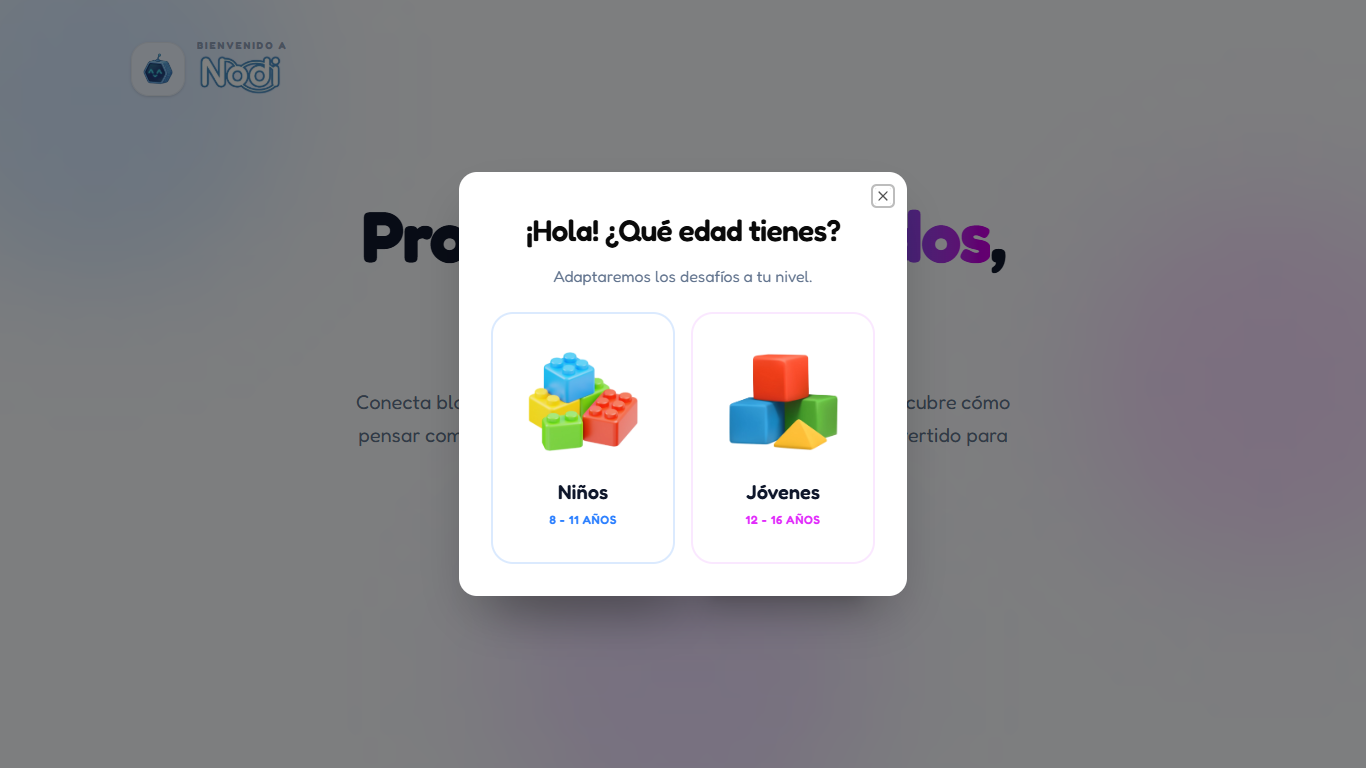
\includegraphics[width=\textwidth]{../images/seleccion-edad.png}
    \caption[Pantalla de selección de rango de edad]{\normalfont Pantalla de selección de rango de edad para la asignación de desafíos}
    \label{fig:seleccion-edad}
\end{figure}

Una vez establecido el perfil del usuario, los niveles se integran en una interfaz en forma de mapa de progreso. Como se aprecia en la figura \ref{fig:desafio-roadmap}, los desafíos se distribuyen secuencialmente a lo largo de un camino ilustrado. Cada parada en este recorrido actúa como un nivel bloqueado o desbloqueado, acompañado de una imagen gráfica representativa de la temática del reto.

\begin{figure}[H]
    \centering
    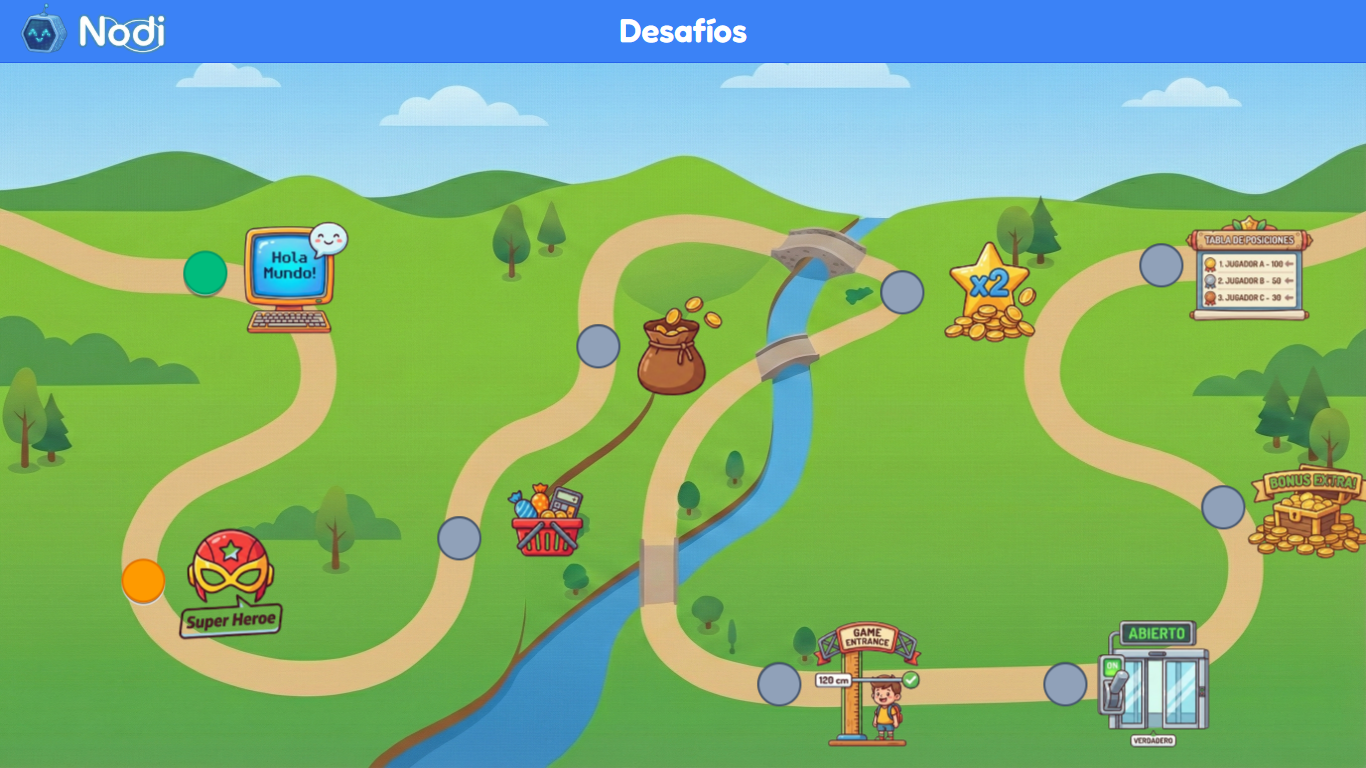
\includegraphics[width=\textwidth]{../images/desafio-roadmap.png}
    \caption[Interfaz del mapa de desafíos]{\normalfont Interfaz del mapa de desafíos}
    \label{fig:desafio-roadmap}
\end{figure}

Esta disposición lúdica ofrece al estudiante un sentido claro de progresión y meta. Al interactuar con cada nodo del mapa, el usuario puede visualizar la descripción y los objetivos específicos del desafío, contando con un botón de acción directa para transicionar hacia la pantalla de resolución del nivel seleccionado.

Al seleccionar un nivel específico desde el mapa interactivo, el estudiante ingresa a la pantalla de resolución del desafío, la cual se ilustra en la figura \ref{fig:editor-desafio}. En esta vista, el concepto de andamiaje cognitivo se hace presente, dado que la paleta de nodos en el panel izquierdo se restringe automáticamente para mostrar únicamente los componentes habilitados para esa misión en particular. Por su parte, el lienzo central se inicializa según el escenario definido, pudiendo presentarse completamente en blanco o desplegar una configuración de nodos iniciales preestablecida, estableciendo así el punto de partida lógico para el estudiante.

Para optimizar el uso del espacio y mantener el enfoque visual en el flujo de datos, el panel de información del reto se diseñó como una tarjeta flotante ubicada en la esquina superior derecha del lienzo. Este panel contiene el estado de la misión, el enunciado con las instrucciones y el botón de acción para probar la solución construida.

El proceso de validación de desafíos se diseñó para ser transparente y formativo. Al accionar el botón “Probar”, el motor de ejecución realiza una corrida interna utilizando casos de prueba definidos en la configuración del nivel. El sistema evalúa el grafo construido por el usuario y contrasta su comportamiento con la salida esperada para cada uno de los casos. Si el flujo lógico es incorrecto, el entorno expone el resultado erróneo obtenido. Si el flujo es correcto, se despliega una animación de celebración y se desbloquea el siguiente nivel en el mapa de desafíos.

\begin{figure}[H]
    \centering
    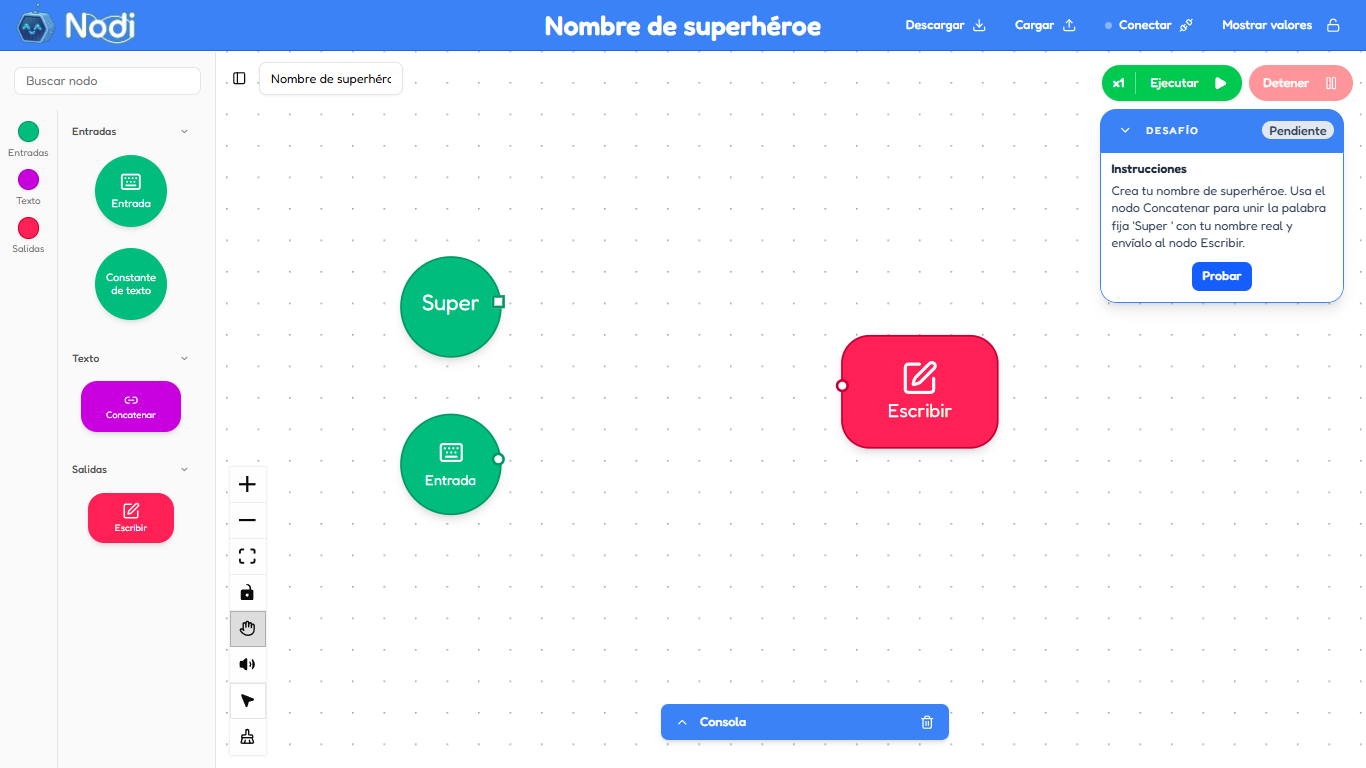
\includegraphics[width=\textwidth]{../images/editor-desafio.png}
    \caption[Interfaz de resolución de desafíos]{\normalfont Interfaz de resolución de desafíos}
    \label{fig:editor-desafio}
\end{figure}

\usubsubsection{Ampliación del modelo de distribución}

Como parte de las mejoras introducidas en el tercer incremento, se realizó un refinamiento sobre las capacidades de ejecución distribuida implementadas en la iteración anterior. Para potenciar la capacidad de los estudiantes de abordar problemas basados en el procesamiento paralelo de datos, se incorporaron nuevos componentes al lenguaje visual tomando como inspiración las operaciones definidas en el estándar de Message Passing Interface (MPI). Adaptando este subconjunto de operaciones colectivas se diseñaron e implementaron los siguientes nodos:

\begin{itemize}
    \item \textbf{Distribuir (Scatter):} Este componente se fundamenta en la operación Scatter de MPI, en la cual un proceso distribuye partes de un arreglo de datos a diferentes procesos. En el contexto del lenguaje, este nodo actúa sobre una estructura de datos tipo lista. Al activarse, fragmenta la colección y enruta sus elementos de manera equitativa hacia los distintos dispositivos o nodos de procesamiento conectados.
    \item \textbf{Reunir (Gather):} Su diseño se basa en la operación Gather de MPI, conceptualizada para que varios procesos envíen partes de un arreglo de datos a un proceso central que las recopila. En el entorno desarrollado, este nodo cumple una función de sincronización; espera a que los múltiples nodos distribuidos concluyan su procesamiento y recolecta los resultados individuales, empaquetándolos nuevamente en una única lista de salida para continuar con el flujo lógico del programa principal.
    \item \textbf{Replicar flujo (Broadcast):} Inspirado en la operación Broadcast de MPI, este nodo permite que un mismo subflujo sea enviado simultáneamente a múltiples nodos de procesamiento. Previo a esta actualización, la paralelización de un mismo algoritmo exigía que el usuario copiara y pegara visualmente el flujo de datos repetidas veces para poder asignarlo de manera individual a cada dispositivo de destino. Esta acción repetitiva podía llegar a saturar el lienzo de trabajo, dificultando la comprensión del programa general. Con la introducción de este nuevo nodo, el flujo se programa una sola vez y simplemente se especifican en el bloque todos los dispositivos que van a ejecutarlo concurrentemente.
\end{itemize}

La inclusión de estos nodos abstrae la complejidad técnica del manejo de múltiples procesos y el paso explícito de mensajes. Esta decisión se fundamenta en los hallazgos de \citeA{rodriguez2024}, quien mostró previamente que los niños son completamente capaces de asimilar conceptos de computación distribuida si se les brindan las abstracciones visuales adecuadas. De esta manera, se permite a los jóvenes modelar e interactuar con conceptos avanzados de paralelismo de datos de forma visual, manteniendo la consistencia del paradigma de flujo de datos y enriqueciendo las capacidades del lenguaje para la programación distribuida.

\usubsubsection{Validación y resultados del incremento}

La validación de este incremento se realizó mediante pruebas funcionales del flujo completo de aprendizaje. Se verificó la correcta segmentación de usuarios, el despliegue secuencial de los niveles en el mapa, la restricción adecuada de la paleta de nodos y la evaluación automatizada de soluciones. También se probaron distintos desafíos del currículo diseñado para comprobar que el sistema de validación identificara tanto soluciones correctas como resultados erróneos, ofreciendo retroalimentación coherente al usuario y asegurando una correspondencia entre la representación visual y la lógica de ejecución.

Por otro lado, en el componente distribuido, se validó el comportamiento funcional de los nodos Distribuir y Reunir sobre listas de datos, confirmando que el sistema podía modelar esquemas de división de carga y consolidación de resultados con una mayor abstracción que en la iteración anterior. Estas pruebas permitieron ratificar la capacidad de agregar nuevas categorías de nodos sin reescribir el motor, consolidando la arquitectura modular del proyecto.

Como resultado del tercer incremento, el entorno dejó de ser únicamente una herramienta de construcción de programas para convertirse también en un espacio de aprendizaje guiado a través de un módulo de desafíos gamificados. Esta ruta formativa estructurada permite revelar funcionalidades avanzadas de forma progresiva, aplicando un principio de andamiaje adaptado al desarrollo cognitivo del público objetivo. Asimismo, el refinamiento de la interfaz bajo principios de "piso bajo" logró minimizar la carga cognitiva en la sintaxis visual, mejorando la claridad del entorno mediante metáforas claras e iconografía significativa. Finalmente, los nodos Distribuir, Reunir y Replicar flujo ampliaron las capacidades del lenguaje para representar computación concurrente y distribuida sobre colecciones de datos de manera más accesible.